\documentclass[tikz,border=8pt]{standalone}
\usepackage[T1]{fontenc}
\usepackage{lmodern}
\usepackage{xcolor}
\usetikzlibrary{arrows.meta,positioning,fit,calc,backgrounds}
\pgfdeclarelayer{background}
\pgfsetlayers{background,main}

\definecolor{ink}{HTML}{334155}
\definecolor{line}{HTML}{64748B}
\definecolor{stagefill}{HTML}{F8FAFC}
\definecolor{datablue}{HTML}{DCEAF8}
\definecolor{agentorange}{HTML}{F6B44B}
\definecolor{knowledgegreen}{HTML}{DFF3E8}
\definecolor{verifyviolet}{HTML}{EDE9FE}
\definecolor{evalred}{HTML}{FDECEC}
\definecolor{sourcecream}{HTML}{FFF4CC}
\definecolor{softgray}{HTML}{F1F5F9}

\tikzset{
  font=\sffamily,
  stage/.style={
    draw=line,
    line width=0.65pt,
    fill=stagefill,
    inner xsep=5mm,
    inner ysep=7mm
  },
  stage title/.style={
    font=\sffamily\bfseries\large,
    text=black,
    fill=stagefill,
    inner xsep=2mm,
    inner ysep=0.8mm
  },
  box/.style={
    draw=line,
    line width=0.65pt,
    fill=datablue,
    align=center,
    minimum height=13mm,
    text width=34mm,
    inner sep=3pt
  },
  compact/.style={
    box,
    minimum height=11mm,
    text width=28mm,
    font=\sffamily\footnotesize
  },
  widebox/.style={
    box,
    text width=45mm
  },
  small/.style={
    font=\sffamily\footnotesize,
    text=ink
  },
  orange/.style={box, fill=agentorange},
  cream/.style={box, fill=sourcecream},
  green/.style={box, fill=knowledgegreen},
  violet/.style={box, fill=verifyviolet},
  redbox/.style={box, fill=evalred},
  graybox/.style={box, fill=softgray},
  arrow/.style={
    -{Latex[length=2.4mm]},
    draw=ink,
    line width=0.75pt
  },
  feedback/.style={
    -{Latex[length=2.4mm]},
    draw=ink,
    dashed,
    line width=0.75pt
  },
  observe/.style={
    -{Latex[length=2.1mm]},
    draw=ink,
    dotted,
    line width=0.75pt
  },
  route/.style={
    rounded corners=2pt
  },
  flowlabel/.style={
    font=\sffamily\scriptsize,
    text=ink,
    fill=white,
    inner sep=1.2pt
  },
  side label/.style={
    rotate=90,
    font=\sffamily\Large,
    text=ink,
    align=center
  },
  side rule/.style={
    draw=ink,
    line width=0.7pt
  }
}

\begin{document}
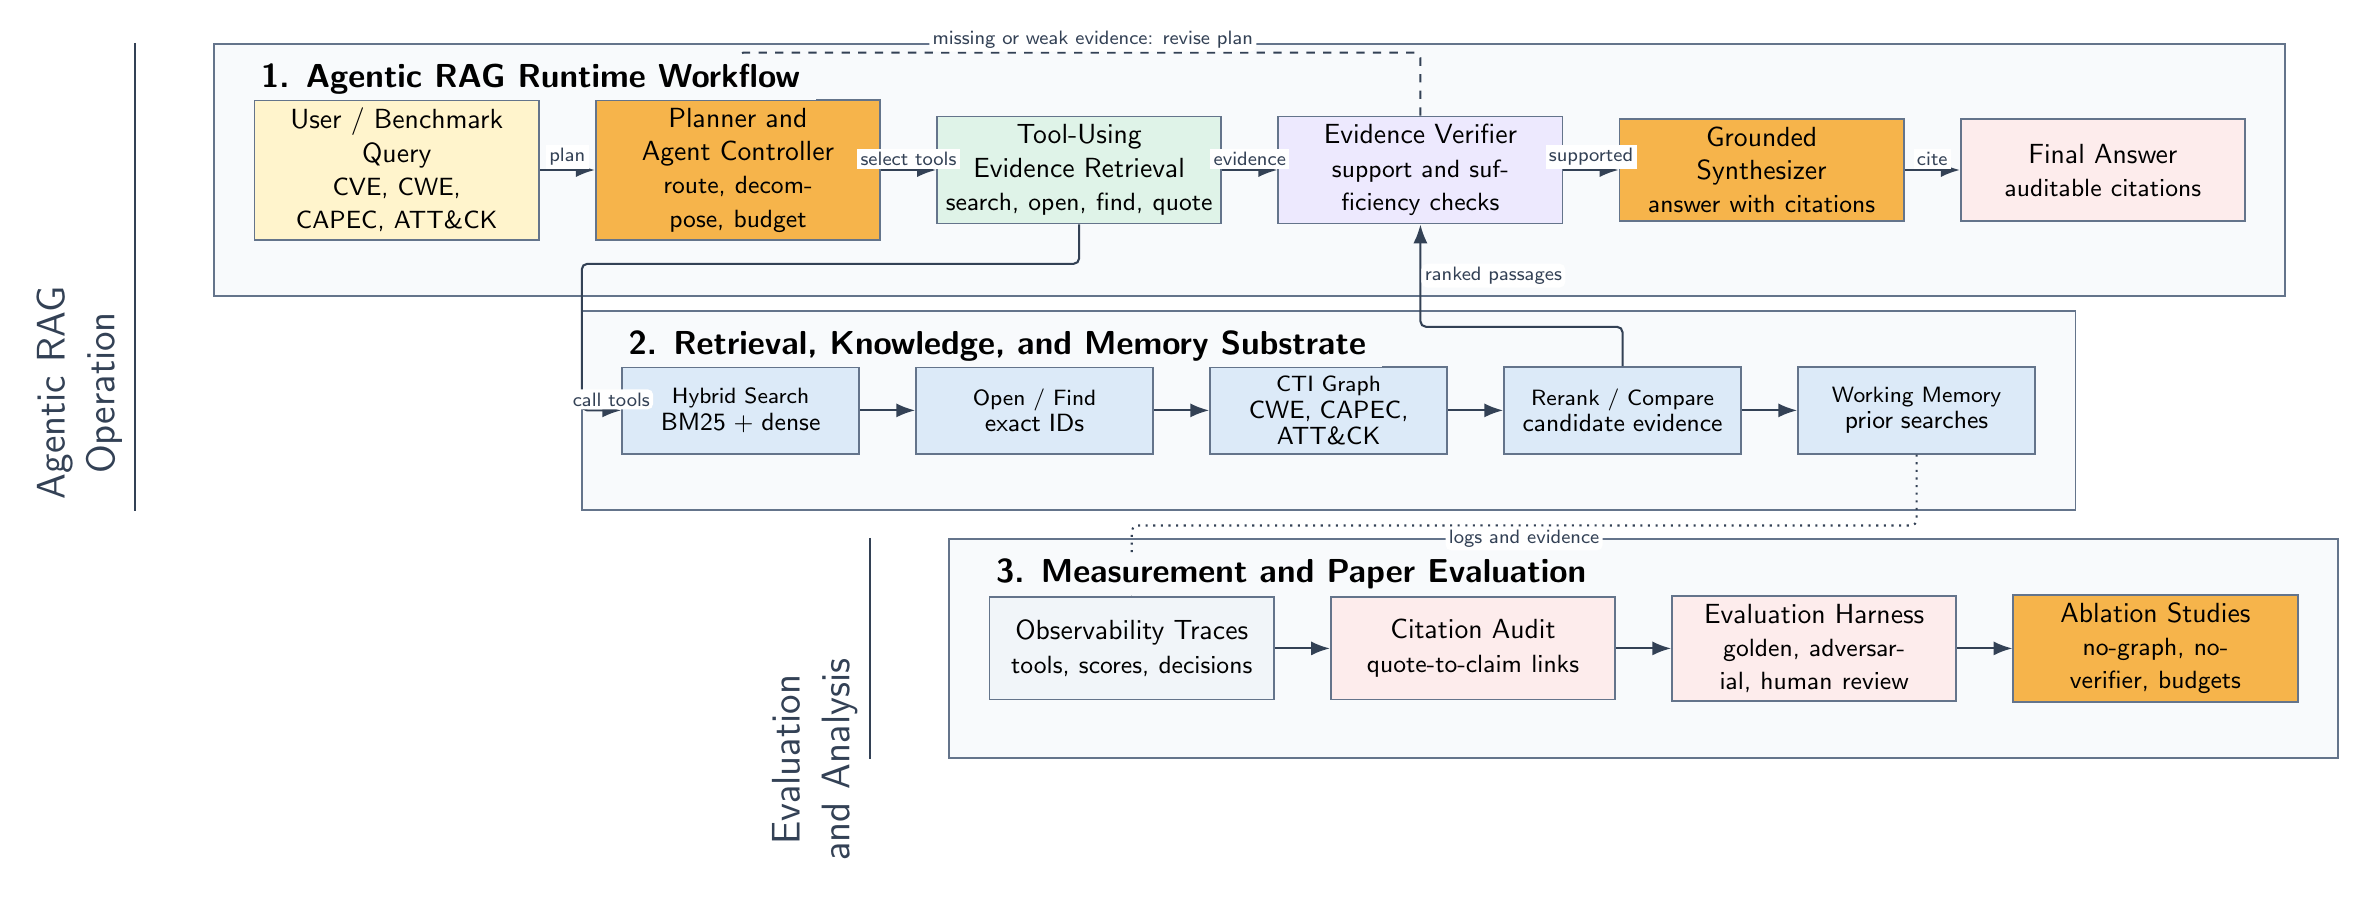
\begin{tikzpicture}[node distance=7mm and 7mm]

% ---------------------------------------------------------------------------
% 1. Runtime agent workflow
% ---------------------------------------------------------------------------
\node[cream] (query) at (0,0) {User / Benchmark\\Query\\{\small CVE, CWE, CAPEC, ATT\&CK}};
\node[orange, right=of query] (planner) {Planner and\\Agent Controller\\{\small route, decompose, budget}};
\node[green, right=of planner] (tools) {Tool-Using\\Evidence Retrieval\\{\small search, open, find, quote}};
\node[violet, right=of tools] (verifier) {Evidence Verifier\\{\small support and sufficiency checks}};
\node[orange, right=of verifier] (synth) {Grounded\\Synthesizer\\{\small answer with citations}};
\node[redbox, right=of synth] (answer) {Final Answer\\{\small auditable citations}};

\begin{pgfonlayer}{background}
\node[stage, fit=(query)(planner)(tools)(verifier)(synth)(answer)] (runtime) {};
\end{pgfonlayer}

\draw[arrow] (query) -- node[flowlabel, above] {plan} (planner);
\draw[arrow] (planner) -- node[flowlabel, above] {select tools} (tools);
\draw[arrow] (tools) -- node[flowlabel, above] {evidence} (verifier);
\draw[arrow] (verifier) -- node[flowlabel, above] {supported} (synth);
\draw[arrow] (synth) -- node[flowlabel, above] {cite} (answer);

% ---------------------------------------------------------------------------
% 2. Retrieval and knowledge substrate
% ---------------------------------------------------------------------------
\node[compact, below=18mm of tools, xshift=-43mm] (hybrid) {Hybrid Search\\{\small BM25 + dense}};
\node[compact, right=of hybrid] (open) {Open / Find\\{\small exact IDs}};
\node[compact, right=of open] (graph) {CTI Graph\\{\small CWE, CAPEC, ATT\&CK}};
\node[compact, right=of graph] (rerank) {Rerank / Compare\\{\small candidate evidence}};
\node[compact, right=of rerank] (memory) {Working Memory\\{\small prior searches}};

\begin{pgfonlayer}{background}
\node[stage, fit=(hybrid)(open)(graph)(rerank)(memory)] (substrate) {};
\end{pgfonlayer}

\coordinate (hybridIn) at ($(hybrid.west)+(-5mm,0)$);
\draw[arrow, route] (tools.south) -- ++(0,-5mm) -| (hybridIn)
  -- node[flowlabel, above, near end] {call tools} (hybrid.west);
\draw[arrow] (hybrid) -- (open);
\draw[arrow] (open) -- (graph);
\draw[arrow] (graph) -- (rerank);
\draw[arrow] (rerank) -- (memory);
\draw[arrow, route] (rerank.north) -- ++(0,5mm) -| node[flowlabel, near end, right] {ranked passages} (verifier.south);

% Explicit repair loop.
\draw[feedback, route] (verifier.north) -- ++(0,8mm)
  -| node[flowlabel, pos=0.24, above] {missing or weak evidence: revise plan} (planner.north);

% ---------------------------------------------------------------------------
% 3. Measurement sidecar
% ---------------------------------------------------------------------------
\node[graybox, below=18mm of graph, xshift=-25mm] (trace) {Observability Traces\\{\small tools, scores, decisions}};
\node[redbox, right=of trace] (audit) {Citation Audit\\{\small quote-to-claim links}};
\node[redbox, right=of audit] (eval) {Evaluation Harness\\{\small golden, adversarial, human review}};
\node[orange, right=of eval] (ablation) {Ablation Studies\\{\small no-graph, no-verifier, budgets}};

\begin{pgfonlayer}{background}
\node[stage, fit=(trace)(audit)(eval)(ablation)] (measurement) {};
\end{pgfonlayer}

\draw[observe, route] (memory.south) -- ++(0,-9mm)
  -| node[flowlabel, pos=0.25, below] {logs and evidence} (trace.north);
\draw[arrow] (trace) -- (audit);
\draw[arrow] (audit) -- (eval);
\draw[arrow] (eval) -- (ablation);

% Side grouping labels.
\coordinate (opTop) at ($(runtime.north west)+(-10mm,0)$);
\coordinate (opBottom) at (opTop |- substrate.south west);
\draw[side rule]
  (opTop) -- (opBottom)
  node[midway, left=7mm, side label] {Agentic RAG\\Operation};

\coordinate (evalTop) at ($(measurement.north west)+(-10mm,0)$);
\coordinate (evalBottom) at (evalTop |- measurement.south west);
\draw[side rule]
  (evalTop) -- (evalBottom)
  node[midway, left=7mm, side label] {Evaluation\\and Analysis};

% Draw titles last so arrows and dotted traces sit behind text.
\node[stage title, anchor=north west] at ($(runtime.north west)+(4mm,-1.8mm)$)
  {1. Agentic RAG Runtime Workflow};
\node[stage title, anchor=north west] at ($(substrate.north west)+(4mm,-1.8mm)$)
  {2. Retrieval, Knowledge, and Memory Substrate};
\node[stage title, anchor=north west] at ($(measurement.north west)+(4mm,-1.8mm)$)
  {3. Measurement and Paper Evaluation};

\end{tikzpicture}
\end{document}
